\documentclass[bachelor,winfonts]{jnuthesis}

% 论文标题
\titlea{人工智能应用——聊天机器人的}
\titleb{开发}

% 论文作者姓名
\author{谭啸}
% 论文作者学生证号
\studentnum{1030413620}
% 导师姓名职称
\supervisor{徐华}
\supervisorpos{教授}
% 第二行导师姓名职称,仿照第一行填写,没有则留空
\supervisorb{}
\supervisorbpos{}
% 论文作者的学科与专业方向
\major{计算机科学与技术}
% 论文作者所在院系的中文名称,学士学位论文此处不带“学院”二字
\department{物联网}
% 论文作者所在学校或机构的名称。此属性可选,默认值为``江南大学''。
\institute{江南大学}
% 学士学位获得日期,需设置年、月,默认为编译日期。
%\bachelordegreeyear{2017}
%\bachelordegreemonth{6}

\begin{document}

% 制作中文封面
\maketitle

% 开始前言部分
\frontmatter

% 论文的中文摘要
\begin{abstract}

\keywords{小世界理论;网络模型;数据中心}
\end{abstract}

% 论文的英文摘要
\begin{englishabstract}

% 英文关键词。关键词之间用英文半角逗号隔开,末尾无符号。
\englishkeywords{Small World, Network Model, Data Center}
\end{englishabstract}

% 生成论文目录
\tableofcontents

% 开始正文部分
% 大概 30 行,为 1 页。
\mainmatter

\chapter{绪论}\label{chapter_introduction}
\section{聊天机器人的定义及背景}
聊天机器人是什么?聊天机器人是一种通过自然语言模拟人类进行对话的程序。通常运行在特定的软件平台上,如PC平台或者移动终端设备平台,而类人的硬件机械体则不是必需的承载设备。

聊天机器人的研究源于图灵(Alan M. Turing)在1950年《Mind》上发表的文章《Computing Machinery and Intelligence》,文章开篇提出了“机器能思考吗?”的设问,并且通过让机器参与一个模仿游戏来验证“机器”能否“思考”,进而提出了经典的图灵测试。图灵测试被认为是人工智能的终极目标,图灵本人因此也被称作“人工智能之父”。

“聊天机器人”(ChatterBot)这个术语最早由麦可·洛伦·莫尔丁(Michael Loren Mauldin,开发了第一个Verbot,Julia)于1994年时在谈话节目中提及。最早的聊天机器人 ELIZA 诞生于1966年,由麻省理工学院(MIT)的约瑟夫·魏泽鲍姆(Joseph Weizenbaum)开发,用于在临床治疗中模仿心理医生。值得注意的是尽管ELIZA的实现技术仅为关键词匹配及人工编写的回复规则,但魏泽鲍姆本人对ELIZA的表现感到吃惊,随后撰写了《Computer Power and Human Reason》这本书,表达他对人工智能的特殊情感。

为了进一步将图灵测试付诸实践,美国科学家兼慈善家休·勒布纳(Hugh G. Loebner)于1990年设立了人工智能年度比赛——勒布纳奖(Loebner Prize)(包括10万美金的奖金和一块印有勒布纳与图灵头像的金牌)。勒布纳奖的设立旨在奖励首个与人类回复无差别的计算机程序,即聊天机器人系统,并以此推动图灵测试及人工智能的发展。在勒布纳奖的推动下,聊天机器人的研究迎来了一个高潮,这里面较为代表性的聊天机器人系统是ALICE(Artificial Linguistic Internet Computer Entity)\cite{alicewebsite}。受到ELIZA聊天机器人的启发,理查德·华勒斯(Richard S. Wallace)博士在1995年开发了ALICE系统。ALICE曾经在2000年、2001年和2004年三次问鼎勒布纳奖,并于1998年开始开源,目前全世界有超过500个开发者为ALICE项目贡献代码。值得注意的是,随着ALICE一同发布的AIML(Artificial Intelligence Markup Language)目前被广泛应用在移动端虚拟助手的开发中。尽管ALICE采用的是启发式模板匹配的对话策略,但是它仍然被认为是同类型聊天机器人中性能最好的系统之一。而本文研究的内容,也与 ALICE 系统密切相关。


\section{国内外研究现状}
从1995年开始,互联网得到快速发展,各式各样的聊天机器人系统也不断出现在公众视线里。各个公司巨头几乎都着手或已实现自己的机器人。

从技术层面来看,从上一节我们初步得知聊天机器人一开始是基于规则匹配的,即预先将回答存储,然后提取问句中的关键词和主题,通过一定的算法,来查找预先存储好的回答数据库,构建这样的聊天机器人相对简单,目前市面上有很多公司依然是基于类似的算法实现自家聊天机器人的,虽然简单,可效果并不差。

目前深度学习也是另一个极热的热点,基于神经网络的对话模型\cite{seq2seq},打开了聊天机器人开发的另一片天地。这种方式,不再需要检索数据库,而是将输入翻译为输出(图\ref{fig:pic1}),能够自己生成句子。Google 开源了 tensorflow 深度学习框架,可以让普通开发者在本地搭建一个运行深度学习的环境。

\begin{figure}[htbp]
  \centering
  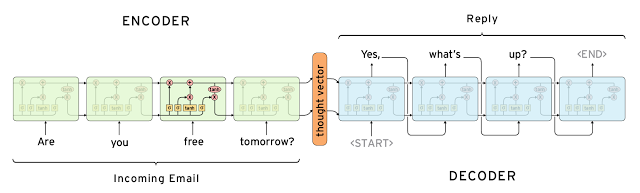
\includegraphics[width= 1\textwidth]{nct-seq2seq.png}\\
  \caption{输入翻译到输出}\label{fig:pic1}
\end{figure}

从应用场景分类来看,比较活跃的有在线客服、公共聊天、个人助理等种类\cite{chinaAI}。在线客服聊天机器人的主要功能是与用户进行基础的沟通,回复用户对公司的产品或者服务的咨询,这样能有效的降低客服的运营成本。应用场景通常为大厅立式终端,或者微信公众号。代表性的系统有京东的JIMI客服机器,银行的咨询和取号机器人等。用户可以通过与JIMI聊天了解商品的详细信息,价格,以及反馈购物中存在的问题等。值得称赞的是,JIMI具备一定的拒识能力,能够知道自己不能回答用户的哪些问题,准确的将此次会话转向人工客服。公共聊天室场景的聊天机器人,能根据聊天主题的改变,以及进入聊天室的用户等因素,做出反应。国外的某些商业网站就有一些有趣的聊天机器人,比如 github 推出的 HUBOT,它更像是一个可配置脚本机器人,能够在特地的聊天室环境,自动完成很多工作,目前已经开源。个人助理类应用主要通过,语音或文字与聊天机器人系统进行交互,实现个人事务的查询及代办功能,如天气查询、空气质量查询、旅游住宿查询、电影片购买、酒店预订、餐饮等,对用户的生活质量带来了很大提升。一般这类机器人都是以 App 的形式使用的,代表性的 App  有百度的小度、新浪微博机器人、Apple的Siri、Google的Now、微软小娜等。Apple的Siri更是为广大果粉津津乐道。Apple的Siri本体集成在 iOS 系统中,用户可以简单的摁下 home 键唤起,支持的交流方式有点触、语音。在 Siri 刚开始发布的时候,受聊天机器人业整体发展水平限制,并没有带来太大的关注,但随着 iOS 系统的迭代和科技的进步,Siri 已经变得非常实用了。

然而,聊天机器人并不是大公司才有的“专利”,一种新兴的服务——聊天机器人平台,让个人用户或小公司,能够以比较低的成本,定制属于自己的聊天机器人。Facebook Messenger 是最流行的消息平台之一,每月拥有 10 亿多活跃用户。在 Facebook 向开发人员开放其机器人平台几个月内,已有 23,000 多名开发人员在构建机器人。目前为止,他们已发布了 18,000 多个机器人。Facebook Messenger 机器人与 Facebook 页面紧密相关,这在企业中非常普遍。Slack 是一个适合工作相关团队的群组消息平台。截至 2016 年 2 月,它每月拥有 230 万活跃用户,而且这一数字正在快速增长。Slack 是当前的聊天机器人复兴浪潮中的先驱之一。Slack 提供了业界第一个 “机器人商店”,使团队能更轻松地发现和安装机器人。不出所料,大部分 Slack 机器人都与工作和生产力有关。国内的微信,每月活跃用户有7亿多,企业通常在建立网站很久以前就已经拥有了微信机器人。


\section{存在的主要问题}
从宏观上来说,目前聊天机器人的实现,依然存在一些公认的难题和挑战。其中包括:如何利用好上下文信息,如何解决通用回复问题以及如何计算一次会话的好坏与质量。

一个好的聊天机器人应该能够结合上下文进行回复。在长对话中,人类可以跟踪说过的人名,地名,心情信息等等。如何有效利用长对话中的信息成为研究的热点问题。聊天机器人中另一个常见的问题是,在基于生成的方法中倾向于生成通用的回复,像“很好”,“我不知道”,这些在大多情况下适用的回复。针对这种问题,很多研究者试图通过改变目标函数来提高回复多样化。如何评价一个模型结果的好坏同样是聊天机器人实现的一个难点。由于在回复中可能会包含完全不同的单词或者短语,因此机器翻译中常用的评估矩阵 ELEU 并不适合用来作为聊天机器人的评价矩阵。

从国内的广泛应用来说,已有的聊天机器人的实现比如 AIML ,基于一些历史原因,API实现并不完美,导致模板规则的编写难度较大,而且 AIML 内置的分词手段是基于空格来分隔英文单词的,而中文没有单词一说,所以必须依赖外部分词工具,因此想使用 AIML 必须改写内部一些代码。

\section{论文主要研究内容}
本文主要工作是剖析 AIML 核心,并实现一个新的版本(Json Robot)。针对目前网络上越来越多的聊天机器人平台的发布,他们有些是基于 AIML 设计的,既需要每个用户都学习晦涩的 AIML 语法,因此设计一个模板书写简洁易懂,并且可配置插件的机器人是一件很有意义的事情。

新版本必须具备 AIML 的基本功能,同时拥有一些创新点,具体对比请看(表\ref{table:t1})。

\begin{table}[ht!]
  \centering
  \begin{tabular}{cp{38mm}p{38mm}}
    \toprule
    \textbf{} & \textbf{Json Robot} & \textbf{AIML}\\
    \midrule
    模板编写  & json文件,key-value的形式,语义化编写 &  xml文件,树状形式,需要阅读大量说明才能编写   \\
    \hline
    支持的功能     & 
    \begin{enumerate}
    \item 基本的匹配规则
    \item 答案随机返回
    \item 重定向搜索
    \item 问与答之间的关系是多对多
    \item 可配置插入第三方模板
    \end{enumerate} &
    \begin{enumerate}
    \item 基本的匹配规则
    \item 答案随机返回
    \item 重定向搜索
    \item 问与答之间的关系是多对多
    \item 基于存储对话关键信息的方式关联上下文
    \end{enumerate} \\
    % \\1.重定向搜索\newline2.答案随机返回\newline3.基本的匹配规则\newline4.问与答之间的关系是多对多\newline5.可配置插入第三方模板  &  1.重定向搜索\newline2.答案随机返回\newline3.基本的匹配规则\newline4.问与答之间的关系是多对多\newline5.基于存储对话关键信息的方式关联上下文   \\
    \hline
    存储形式     & 本地磁盘 + 索引文件    &  通常基于数据库   \\
    \hline
    读取方式及速度     & 通过文件路径打开文件,快     & 连接并查询数据库,慢 \\
    \hline
    内部设计    & 现代API的设计,模块化   &  复杂(可以参考已有的Python实现,同样的功能 Json Robot 所需代码更少)   \\
    外部接口    & 简单   &  简单\\
    \bottomrule
  \end{tabular}
  \caption{AIML和Json Robot对比}\label{table:t1}
\end{table}

本文一共分为六章。

第一章简要介绍了聊天机器人的历史和发展状况,以及面临的挑战。

第二章主要介绍,开发过程中通过查阅的资料而总结的一些理论基础。其中包括学习者特征分析等等理论。

第三章主要介绍了 AIML 的核心匹配算法。AIML 是一个开源机器人,关于它的匹配规则,这篇文章有详细介绍\cite{aiml-match-pattern}。这是程序的核心所在,所有的其他的搜索逻辑都将成为这部分的扩展。

第四章介绍了中文分词。本项目采用的是 Bosonnlp 公司的分词技术,采取调用第三方 Restful API 的形式。该服务能提供的功能其实并不仅仅只有分词,还有关键词提取,情感分析等,这些都是聊天机器人可以利用的增强工具。

第五章介绍了本系统(Json Robot)的详细设计过程。包括系统的前后端架构,编码的模块化,良好的测试保障,以及用户界面的设计等。

第六章是总结。一方面总结了项目的最终实现效果,另一方面对需要增强的地方也提出展望。聊天机器人的热度依旧会持续下去。









\chapter{相关理论基础}


% \begin{itemize}
% \item 模板书写
% \item 这是第二项。这是第二项。这是第二项。这是第二项。这是第二项。这是第二项。这
%   是第二项。这是第二项。这是第二项。这是第二项。这是第二项。
% \item 这是第三项。这是第三项。这是第三项。
%   \begin{itemize}
%   \item 测试第二层列表。测试第二层列表。
%   \item 测试第二层列表。测试第二层列表。
%   \end{itemize}
% \end{itemize}







\chapter{AIML核心机制}
\chapter{中文分词}


\chapter{系统设计与实现}
\chapter{总结与展望}
\section{论文总结}
\section{工作展望}


\begin{acknowledgement}
  首先感谢
\end{acknowledgement}


% 参考文献
\nocite{*}
\bibliography{bachelor}
%%%%%%%%%%%%%%%%%%%%%%%%%%%%%%%%%%%%%%%%%%%%%%%%%%%%%%%%%%%%%%%%%%%%%%%%%%%%%%%
\end{document}